\section{Spectrum and learning dynamics}
\label{sec:dynamics}

\begin{figure*}[t]
\centering
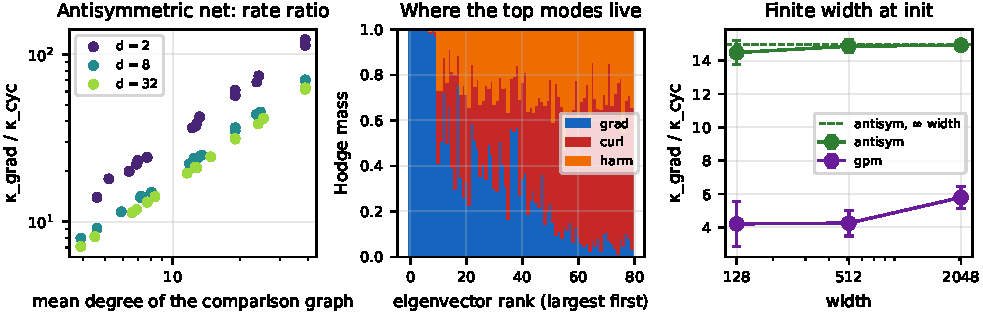
\includegraphics[width=\textwidth]{figures/spectrum.pdf}
\caption{Edge NTK of the antisymmetric network. Left: ratio of the mean kernel
eigenvalue on gradient flows to that on cyclic flows, over \SpeNGraphs\ random
comparison graphs (sizes 20 and 40, densities 0.15--1, depth 1 shown), against
the mean degree; colour is the feature dimension. Middle: Hodge composition of
the top 80 eigenvectors on a \SpeCanonN-item graph (\SpeCanonE\ edges;
gradient/curl/harmonic dimensions \SpeCanonGradDim/\SpeCanonCurlDim/\SpeCanonHarmDim).
Right: the same ratio for the empirical kernel at initialisation versus width,
with the infinite-width value dashed; GPM is shown for comparison.}
\label{fig:spectrum}
\end{figure*}

\paragraph{The spectrum is ordered.} Figure~\ref{fig:spectrum} confirms H1
for the gradient-versus-cycle split. In every one of the \SpeNGraphs\ graphs
the antisymmetric kernel's gradient rate exceeds its cyclic rate, by
\SpeRatioMin$\times$ on the sparsest graphs to \SpeRatioMax$\times$ on
complete ones (mean \SpeRatioSparse$\times$ at density 0.15,
\SpeRatioDense$\times$ at density 1), and the ratio grows with the mean
degree, as the additive-part argument predicts. Low feature dimension and
shallow networks sharpen it (\SpeRatioLowD$\times$ at $d=\SpeLowD$ versus
\SpeRatioHighD$\times$ at $d=\SpeHighD$; \SpeRatioDepthOne$\times$ at depth 1
versus \SpeRatioDepthTwo$\times$ at depth 2), since both enlarge the
interaction part of the kernel. The top ten eigenvectors carry
\SpeTopTenGradMass\% of their mass in gradient space. At finite width the
empirical kernel reproduces the analytic ratio already at width
\SpeEmpWLo\ (\SpeEmpAntisymWLo\ versus \SpeAnaRatioCanon), and the kernels agree
entrywise to \SpeEmpErrHi\% at width \SpeEmpWHi. GPM is ordered too but less
sharply (\SpeEmpGpmWLo--\SpeEmpGpmWHi$\times$): its bilinear form has no
additive part to amplify rankings.

\paragraph{Curl and harmonic are not ordered.} The second half of H1 fails.
The ratio of curl to harmonic rates ranges from \SpeCurlHarmMin\ to
\SpeCurlHarmMax\ with mean \SpeCurlHarmMean: the network does not distinguish
cycles around triangles from cycles around holes. This matches the argument
above --- both live only in the interaction part --- and it is where our
setting differs from the Topological NTK, whose message passing is built on
the Hodge Laplacian itself \cite{krishnagopal2026topological}.

\begin{figure*}[t]
\centering
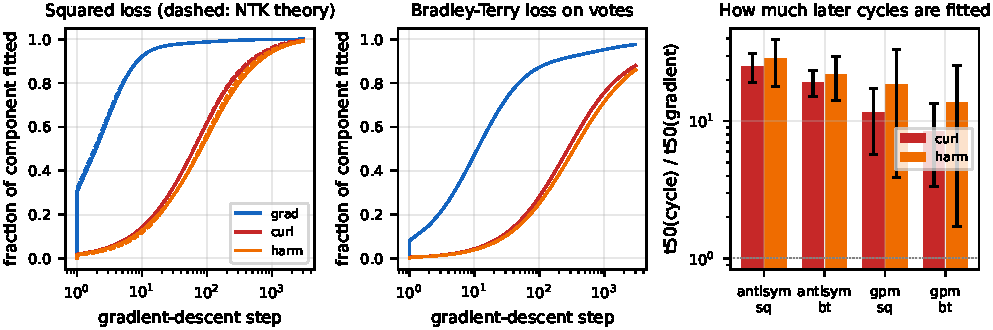
\includegraphics[width=\textwidth]{figures/dynamics.pdf}
\caption{Fraction of each Hodge component of the true flow fitted during
training (antisymmetric net, one seed). Left: squared loss, with the
linearised NTK prediction dashed. Middle: Bradley--Terry loss on 200 votes per
edge. Right: how many times later the cyclic components reach 50\% than the
gradient component, over seeds, for the antisymmetric net and GPM under both
losses.}
\label{fig:dynamics}
\end{figure*}

\paragraph{Training follows the spectrum.} On a synthetic task
(\TaskN\ items, $d=\TaskD$, density \TaskDens; the true preference combines a
smooth utility and a skew interaction, giving
\TaskFracGrad/\TaskFracCurl/\TaskFracHarm\% gradient/curl/harmonic energy),
Figure~\ref{fig:dynamics} shows H2. The antisymmetric network fits the
ranking in a handful of steps and the cycles \DynAntisymSqCurl$\times$ (curl)
and \DynAntisymSqHarm$\times$ (harmonic) later under the squared loss, and
\DynAntisymBtCurl$\times$ and \DynAntisymBtHarm$\times$ later under the
Bradley--Terry loss on votes; GPM shows the same order with a smaller gap
(\DynGpmSqCurl$\times$ and \DynGpmSqHarm$\times$). The order held in
\DynOrderOk\ of \DynOrderTotal\ runs. Under the squared loss the linearised
NTK prediction tracks the network's per-component fit to within \DynLinDev\
at every step --- the dynamics \emph{is} the spectrum. The scalar model fits
the ranking just as fast and never moves on cycles (final curl fit
$\le\DynScalarCurlFinal$), which costs it on held-out pairs: \DynHoScalar\
sign accuracy versus \DynHoAntisym\ (antisymmetric) and \DynHoGpm\ (GPM),
because the true preferences are partly cyclic.

\begin{figure*}[t]
\centering
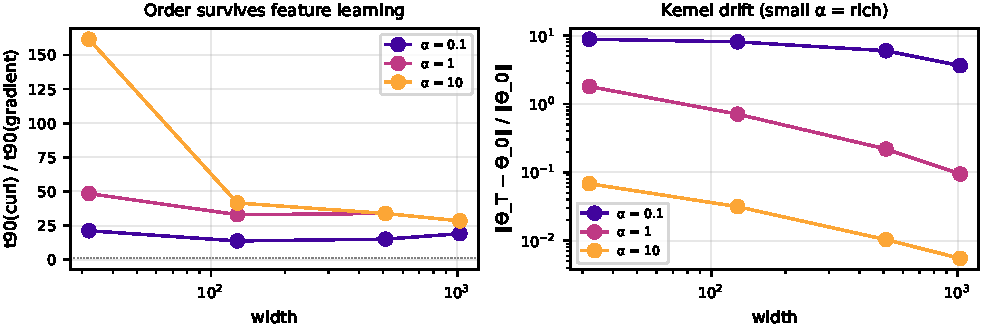
\includegraphics[width=0.8\textwidth]{figures/width.pdf}
\caption{Antisymmetric net across width and output scale $\alpha$ (small
$\alpha$ = rich, feature learning). Left: how many times later curl reaches
90\% than the gradient part. Right: relative change of the empirical kernel
over training.}
\label{fig:width}
\end{figure*}

\paragraph{Feature learning narrows the gap but keeps the order.}
Figure~\ref{fig:width} moves the network out of the kernel regime. With
$\alpha=\WidAlphaLazy$ the kernel barely moves (relative drift
\WidDriftLazy) and curl reaches 90\% \WidRatioLazy$\times$ after the ranking;
with $\alpha=\WidAlphaRich$ the kernel changes by a factor of
\WidDriftRich\ and the gap shrinks to \WidRatioRich$\times$, because the
evolving kernel becomes less ordered (final rate ratio \WidKRatioRich\ versus
\WidKRatioLazy). The order held in all \WidOrderOk\ of \WidRuns\ runs across
widths \WidMin--\WidMax. Feature learning here also generalises slightly
better (held-out \WidAccRich\ versus \WidAccLazy): it learns the cycles sooner.
